\chapter{Conclusions~and~Future~Work}
\label{chap:future} 


\section{Future work}
\subsection{Ensemble training and uncertainty estimation}

There exist a number of uncertainty measures, specifically developed for object detection, based on Bayesian \gls{NMS} \cite{Harakeh}, test time augmentation {Wei2018} and, of particular interest, ensembles \cite{Le2018}. Some discussion of this is in section--\ref{sec:example_selection}. 

K-fold cross-validation is proposed as a future method to improve data usage. It can be used for ensemble-based predictions on new images with uncertainty estimation, unbiased reviewing and machine-assisted verification to check for mistakes, and enhanced accuracy in testing by testing against the full dataset.

In conflict with our desire to use high-resolution images for annotation clarity, ensembles, example selection, and interface responsiveness would all benefit from the use of lower resolution images. More experimentation is necessary to determine the best tradeoff, which seems likely to depend on the dataset.

\subsection{Domain specific applications, counting wildlife}

One promising application for \gls{VBA} has been in counting wildlife, where the annotation tool has been used for verified counting of Antarctic wildlife. Several limitations were discovered, such as efficiency issues with the user interface in the presence of very large numbers of annotations, and the difficulties created by the artificial splitting of images. Addressing efficiency is very straightforward, but a way of allowing the user to divide up very large images would seem beneficial.

Several metrics and image selection heuristics were added to attempt to aid experimentation with time series images. Expanding on these heuristics and providing better methods for exploring and sorting images would be beneficial for studying time series. Adding image level classification would also be useful for sorting and managing datasets. For example, automatically discarding images with poor visibility would be possible if discarded images are labelled and used for learning.

\subsection{Higher level forms of object detection}

\begin{figure}[h!]
\begin{subfigure}[t]{1.0\linewidth}
  \centering
  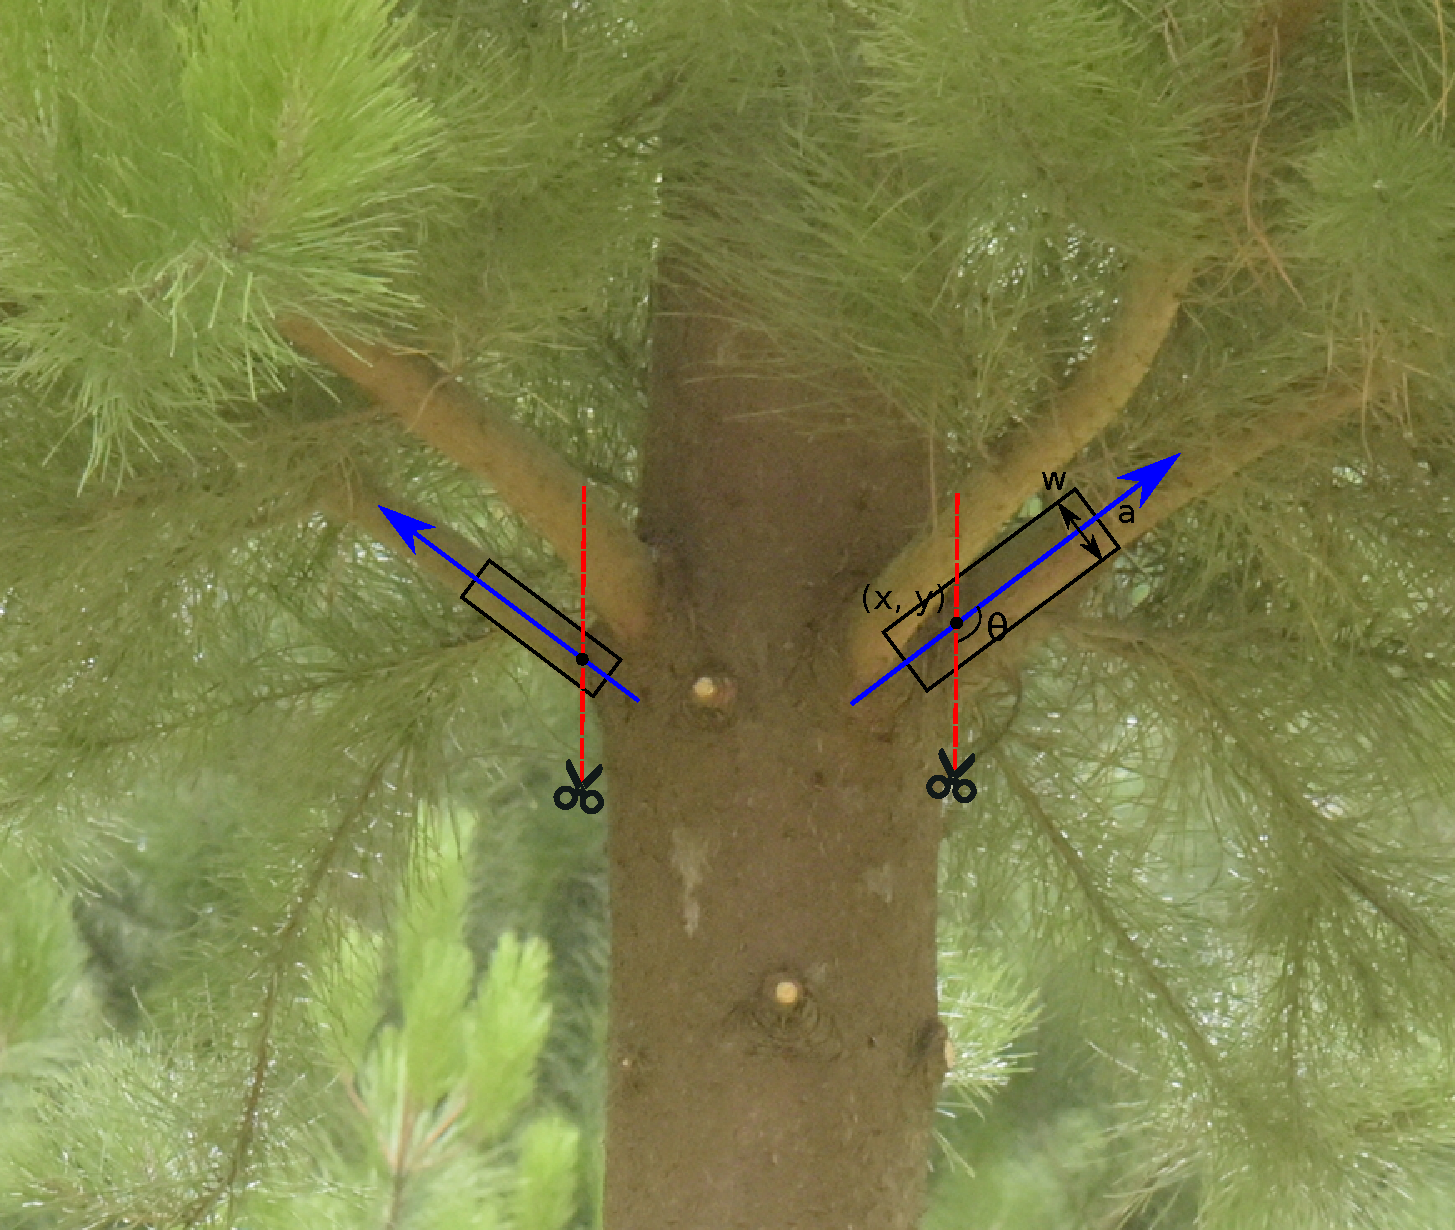
\includegraphics[width=0.8\linewidth]{figures/future/tree_cutpoint.pdf}
  \caption{} 
\end{subfigure}

\begin{subfigure}[t]{1.0\linewidth}
  \centering
  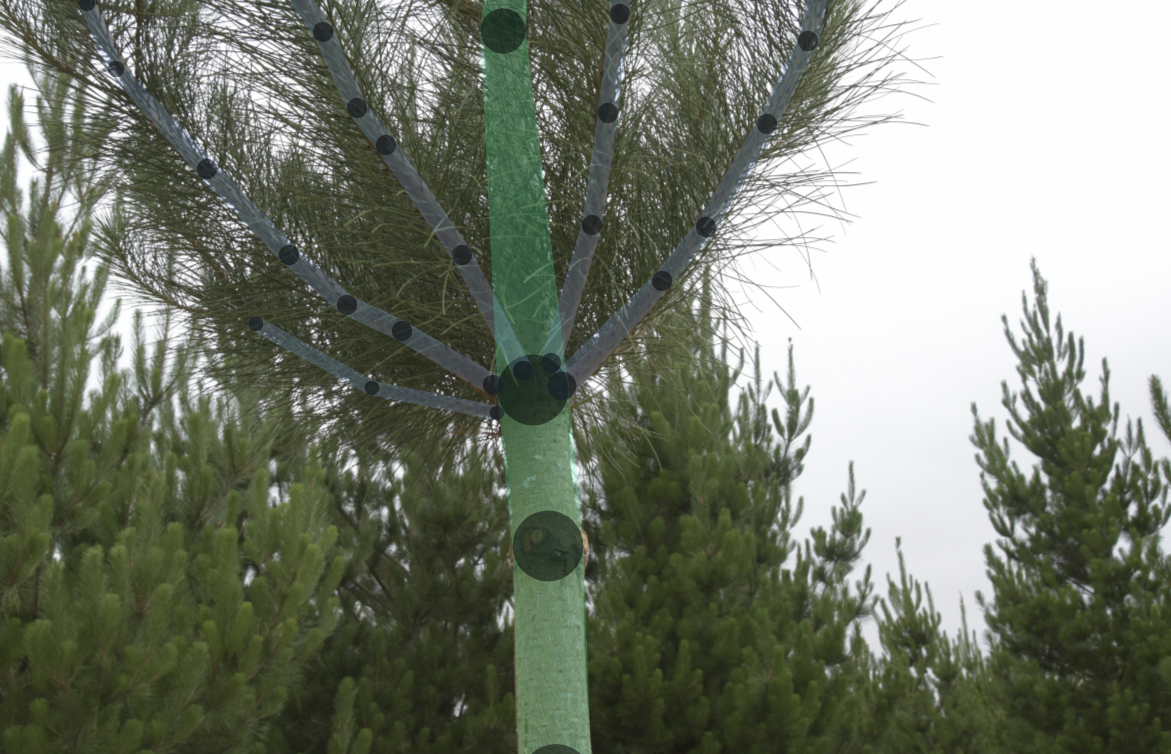
\includegraphics[width=0.8\linewidth]{figures/future/tree_branches.jpg}
  \caption{} 
\end{subfigure}
\caption{Ongoing work into annotating trees in (a) cut-point detection, (b) tree structure skeleton extraction }
\label {fig:future_trees}
\end{figure}

Bounding boxes have limits for object detection; they only very loosely fit an object, and some objects cannot be described well by bounding boxes at all. Tree branches are fit by bounding boxes very poorly; they're very long, and it's not always clear where they start and stop. Future work will focus on other kinds of object detection, and the ability to pick the type for the task at hand.

Recent work in object detection \cite{Zhou2019} or \cite{Law2018}, both successors to the RetinaNet detector \cite{Wang2017} used in this work, have shown that both the anchor box approach and \gls{NMS} is unnecessary. In \cite{Zhou2019}, local maxima in a single heat map are used to detect objects, and all other parameters are regressed, allowing for the simple extension to a range of different types of object detector by regressing different properties.

The branches dataset used as an example in this work, is a trial for detecting cut positions. Figure~\ref{fig:future_trees} shows two directions in the annotation of tree structures, cut point estimation and skeletal extraction for robotic pruning applications. Skeleton estimation on tree structures can be adapted from methods used for road network extraction \cite{Li2018}, shape estimation \cite{Jiang2019a} or polygon extraction \cite{Acuna2018}, and can work well within the \gls{VBA} approach.

\subsection{Annotating uncertainty}

In future, the ability to annotate images based on uncertainty may be a useful approach, as a means of calibrating confidence and for weighting examples in the training process. As opposed to epistemic uncertainty, aleatoric uncertainty can be estimated directly (by a \gls{NN}, for example, by regression).  

This kind of uncertainty annotation may also be useful in weighting training loss, where the network can place more weight on hard, yet unambiguous examples. The use of Focal Loss means that examples which fail to classify well are weighted much more highly. If these examples are ambiguous because of shadow or lack of resolution - their contribution to the training is noise.

Hard examples are often cited as being the most useful for an object detector, but if the hard examples are not really hard examples, because they are also visually ambiguous or uncertain (high aleatoric uncertainty) then their usefulness as a learning target might be less, but still possesses value for use in validation and calibration.



\subsection{User verification and testing}
\label{sec:user_verification}

The risk of algorithmic bias brings into question the quality of a dataset annotated with a \gls{VBA} system.  To combat algorithmic bias when a human annotator becomes fatigued, it is proposed that a certain level of \emph{generated} mistakes can be included. The user may be forced to fix the error before they can continue, or statistics from fixing added errors may be used as a measure of the user's trustworthiness. Examples of generate mistakes include false positives, false negatives by removing very high confidence detection, or localisation errors by transform box of high confidence detection. 


\subsection{Software improvements}

There is a range of general software improvements to improve usability and prepare for release to a broader audience. Some plans are detailed in chapter~\ref{chap:design}, including: (a) streamlining detection to avoid the need for selecting manual thresholds, (b) simplifying the interface, (c) easy deployment to cloud-based systems, and (d) integrating and exposing object detection configuration parameters to the user interface and integration of visualisation for metrics.

\section{Conclusion}
\label{sec:conclusion}
\glsresetall

Primarily, out of frustration with the difficulty of capturing and annotating image data, the goal of this thesis became how to effectively annotate images to use machine learning models on new domains in visual recognition. Specifically, the goal has been to evaluate and characterise the best use of a \emph{human-in-the-loop} annotation method I have termed \gls{VBA}, where a machine learning model is trained interactively based on verifying and correcting predictions from a \gls{CNN} based visual recognition model. A key point of difference to similar works developed, either prior or concurrently to this work, is the focus on online training, where existing works use either (a) strong models trained on large data sets or (b) staged systems with alternating periods of annotation and training. 

Chapter~\ref{chap:focus} looked at how image cropping affected classification performance using a \gls{CNN}, a prelude to later work, which examined annotation noise in object detection. For an instance recognition dataset,  a tight cropping and increased resolution were both strongly beneficial to classification using a \gls{CNN}.

In chapter~\ref{chap:metric}, a novel form of mini-batch deep \gls{NCA} metric learning was presented, using a multi-way comparison between feature vectors of each image in a mini-batch. The method worked well for specific cases of \gls{KNN} classification on two instance recognition datasets, however, was very sensitive to parameter changes. It surprisingly worked much better for small batch sizes, where fewer examples are compared at once. 

Chapter~\ref{chap:bootstrap} is an exploratory work into different forms of machine-assisted segmentation. Several methods were examined using segmentation of tree trunks as a test case. The most promising direction was a method of incrementally training a model while annotating by verifying and correcting machine predictions. Experiments showed that by using fine-tuning, surprisingly little data and training time was necessary to achieve workable levels of accuracy to assist annotation. 

Chapter~\ref{chap:design} describes the design and implementation of an object detection system on real-world data of a \gls{VBA} system (for object detection) using lessons learned from chapter~\ref{chap:bootstrap}. I developed an annotation system built around \gls{VBA},  designed for experimentation and rapid prototyping on new domains.  I chose a web-based interface for easy deployment. A novel method for utilising weak detections, which may be well localised even if not classified correctly, was developed (and usage justified in chapter~\ref{chap:annotation}). Additionally, I prototyped a method for using the machine model to aid in reviewing existing annotations.

The \gls{CNN} object detector used in the \gls{VBA} annotation tool is described in chapter~\ref{chap:object_detection}. To accommodate the needs of online training for image annotation (as opposed to necessarily the strongest or fastest object detector), I make some changes to standard practice. Modifications include avoiding weight sharing in object classifiers of different scales, a non-normalised loss function to cope with purely negative images (no objects),  options for cyclical learning rates, and methods for incrementally training and inference using high-resolution images developed. 

The second part of chapter~\ref{chap:object_detection} is devoted to testing the assumptions made in developing the \gls{VBA} tool, on a selection of small-scale datasets annotated for this work. Cyclical learning rates were found to have less impact than assumed. Methods for training, using high-resolution images, were shown to be both practical and deliver improved accuracy at the cost of time; however, training time is plentiful compared to annotation time. Finally, I study the effect of noise (introduced by rough annotation) and systematic bias (such as that caused by algorithmic bias) on object detection. In the presence of either a small amount of either bias or noise, the object detector is quite robust. With reduced data, the sensitivity to noise and systematic bias increases with the additional problem of overfitting. The annotator (and annotation tool developer) should focus on accurate annotation, especially at the beginning of the process. 

Chapter~\ref{chap:annotation} presents a series of studies, where $10$ different and widely varied real-world image sets were annotated to evaluate and explore where the \gls{VBA} system is most applicable. The accuracy of the object detector and the types of user actions were broken down and visualised over annotation time. I analysed the statistics of corrected boxes and attempted to find the human threshold for localisation, a peak of localisation corrections could be seen at around an \gls{IOU} of $0.80$ to $0.85$, depending on the dataset. Therefore, this level of agreement can be used as an approximate benchmark to define a human-level of localisation accuracy.

Image sets with a large degree of uniformity, with many easy cases in each image (as are most datasets used in this work), can be seen to be excellent candidates for \gls{VBA}. Machine provided detections (used unmodified) vary between $75\%$ to $94\%$ of the final annotations (except the \emph{scallops} dataset, at $62\%$). In a few cases, another $10\%$ of annotations were added by confirming weak detections. Most of the datasets annotated, showed improved rates of annotation as annotation progressed, often showing annotation rates faster than would be possible manually, in some cases even from near the beginning of the annotation process. 

Limitations include the current object detector, which struggles with objects which overlap; the human annotator can mainly end up correcting artefacts of the object detector. The \gls{VBA} approach may be useful in those datasets which are less uniform, however it is hypothesised, they may benefit from either (a) a more considerable annotation effort (to reach the same degree of prediction accuracy) or (b) the use of image selection (such as active learning) to select the best images for annotation.

Verified counting of wildlife was shown to be an ideal application for the \gls{VBA} system. Two domains were studied, the first being counting on an Ad\'elie penguin survey, where an established system of verified counting has been used for several years (based on traditional computer vision). My approach, using a \gls{CNN}, has the obvious benefit of being adaptable to new conditions and entirely new problems other than counting Ad\'elie penguins. The second domain was analysing movement patterns of Weddell seal populations in time series images, where a large number of seals can be counted by annotating only a tiny fraction of the total images. Crowd sourcing approaches had previously been used to count the same images, however, my method can achieve similar results with significantly reduced labour and improved consistency. Verified counting is also not mutually exclusive and could be used \emph{with} crowd sourcing to better utilise volunteer time.

Future work will focus on several areas (amongst other smaller goals): (a) different forms of object detection, for example, polygons, oriented boxes and pose estimation; (b) improve the software for broader release, and easy deployment on cloud services; (c) improved use of data, using k-fold cross validation ensembles for uncertainty estimation; (d) application to larger scale annotation tasks, and multi-user annotation.

Overall this work has shown Verification Based Annotation to be a practical method for machine-assisted annotation and combines well with the ability to explore and manage image data to be a useful tool for experimentation in new domains. It is especially effective in image sets with uniformity of object instances, and in combination with active learning should help in situations of less uniform images. In addition to being practical, the interactivity brings improvement in user engagement where the chore of annotating many images becomes the interesting task of teaching a machine to recognise the objects.
